\documentclass[11pt,a4paper,oneside,openright,titlepage,
  headinclude,footinclude,BCOR5mm,
  numbers=noenddot,cleardoublepage=empty,
  tablecaptionabove, dottedtoc,
  bibliography=totoc]{scrreprt}
\usepackage{subfig}
\usepackage[
    eulerchapternumbers,
    subfig,
    beramono,
    eulermath,
    pdfspacing
  ]{classicthesis} 
\usepackage{arsclassica}
\usepackage{graphicx}
\usepackage[norsk,american]{babel}
\usepackage[utf8]{inputenc}
\usepackage[T1]{fontenc}
\usepackage{pdfpages}
\usepackage{titlesec}

$if(natbib)$
\usepackage[$natbiboptions$]{natbib}
\bibliographystyle{$if(biblio-style)$$biblio-style$$else$plainnat$endif$}
$endif$
$if(biblatex)$
\usepackage[$if(biblio-style)$style=$biblio-style$,$endif$$for(biblatexoptions)$$biblatexoptions$$sep$,$endfor$]{biblatex}
$for(bibliography)$
\addbibresource{$bibliography$}
$endfor$
$endif$

% *******************************************************
% DEFINE VARIABLES
% *******************************************************
\newcommand{\myName}{$author.name$}
\newcommand{\myTitle}{$title$}
\newcommand{\mySubTitle}{$subtitle$}
\newcommand{\myLocation}{\spacedlowsmallcaps{$location$}}
\newcommand{\myGroup}{$author.affiliation$}
\newcommand{\myUrl}{\url{$author.homepage$}}
\newcommand{\myTime}{2019, July}
\newcommand{\docsite}{\url{$docsite$}}
\newcommand{\email}{\mail{$author.email$}}

% *******************************************************
% CUSTOMIZATIONS
% *******************************************************
\newcommand{\mail}[1]{\href{mailto:#1}{\texttt{#1}}}
\titleformat{\part}[display]
  {\normalfont\centering\large}%
  {\thispagestyle{empty}\partname~\MakeTextUppercase{\thepart}}{1em}%
  {\color{Maroon}\spacedallcaps}

\begin{document}
\pagenumbering{Roman}
\pagestyle{plain}
% *******************************************************
% Title Front
% *******************************************************
\begin{titlepage}
  \pdfbookmark{Titlepage}{Titlepage}
  \null\vfill
  \begin{center}
    \large \sffamily
    \bigskip
    {\Large\spacedlowsmallcaps{\myName}} \\
    \bigskip
    {\huge\spacedlowsmallcaps{\myTitle} \\}
    \bigskip
    \vspace{9cm}
    \begin{tabular} {cc}
      \parbox{0.3\textwidth}{
\includegraphics[width=3.5cm]{Logo}}
      & \parbox{0.7\textwidth}{{\Large\spacedlowsmallcaps{\mySubTitle}} \\ 
      {\normalsize
      \myGroup \\
      \myUrl \\
      \myTime}}
    \end{tabular}
  \end{center}
  \vfill
\end{titlepage}

% *******************************************************
% Title Back
% *******************************************************
\thispagestyle{empty}
\hfill \vfill
\noindent\myName:
\textit{\myTitle,} \mySubTitle,
\textcopyright\ \myTime.
\medskip
\noindent{\spacedlowsmallcaps{Website}}: \\
\docsite

\medskip
\noindent{\spacedlowsmallcaps{E-mail}}: \\
\email

\vspace{1cm}
\hrule
\bigskip

\noindent $title-abstract$

\pagestyle{scrheadings} 
\clearpage

% *******************************************************
% ABSTRACT
% *******************************************************
$if(abstract)$
\pdfbookmark{Abstract}{Abstract}
$if(summary)$
\begingroup
\let\clearpage\relax
\let\cleardoublepage\relax
\let\cleardoublepage\relax
$else$
\clearpage
$endif$

\addchap{Abstract}
$abstract$
\vfill
$endif$

% *******************************************************
% SUMMARY
% *******************************************************
$if(summary)$
$if(abstract)$
\clearpage
$endif$
\pdfbookmark[1]{Sommario}{Sommario}
\addchap{Summary}
$summary$
$if(abstract)$
\endgroup
$endif$
\vfill
$endif$

% *******************************************************
% ACKNOWLEDGMENT
% *******************************************************
\pdfbookmark{Acknowledgements}{Acknowledgements}

\begingroup
\let\clearpage\relax
\let\cleardoublepage\relax
\let\cleardoublepage\relax

\addchap{Acknowledgements}

$acknowledgement$

\endgroup

% *******************************************************
% Contents
% *******************************************************
\clearpage
\phantomsection
\pdfbookmark{\contentsname}{tableofcontents}
\setcounter{tocdepth}{2}
\begingroup 
  \let\clearpage\relax
  \let\cleardoublepage\relax
  \tableofcontents
\endgroup
\markboth{\spacedlowsmallcaps{\contentsname}}
{\spacedlowsmallcaps{\contentsname}} 

\begingroup 
  \let\clearpage\relax
  \let\cleardoublepage\relax
\endgroup

\cleardoublepage
% *******************************************************
% BODY START
% *******************************************************
\pagenumbering{arabic}


$body$

% *******************************************************
% BIBLIOGRAPHY START
% *******************************************************
$if(natbib)$
$if(bibliography)$
$if(biblio-title)$
$if(has-chapters)$
\renewcommand\bibname{$biblio-title$}
$else$
\renewcommand\refname{$biblio-title$}
$endif$ % has-chapters
$endif$ % biblio-title
$if(beamer)$
\begin{frame}[allowframebreaks]{$biblio-title$}
  \bibliographytrue
$endif$ % beamer
  \bibliography{$for(bibliography)$$bibliography$$sep$,$endfor$}
$if(beamer)$
\end{frame}
$endif$ % beamer
$endif$ % bibliography
$endif$ % natbib


$if(biblatex)$
$if(beamer)$
\begin{frame}[allowframebreaks]{$biblio-title$}
  \bibliographytrue
  \printbibliography[heading=none]
\end{frame}
$else$
\printbibliography$if(biblio-title)$[title=$biblio-title$]$endif$
$endif$ % beamer
$endif$ % biblatex

$if(nociteall)$
\nocite{*}
$endif$

% *******************************************************
% PAPER START
% *******************************************************
\appendix
\part*{Research Papers}
$for(papers)$
\par\chapter{$papers.title$}
\includepdf[pages=-]{$papers.path$}
$endfor$
% \par\chapter{Paper1: A tool for simulating multi-response linear model data}
% 
\includepdf[pages=-]{papers/001.pdf}
% \par\chapter{Paper2:  Model and estimators for partial least squares regression}
% 
\includepdf[pages=-]{papers/002.pdf}
% \par\chapter{Paper3: Comparison of Multi-response Prediction Methods}
% 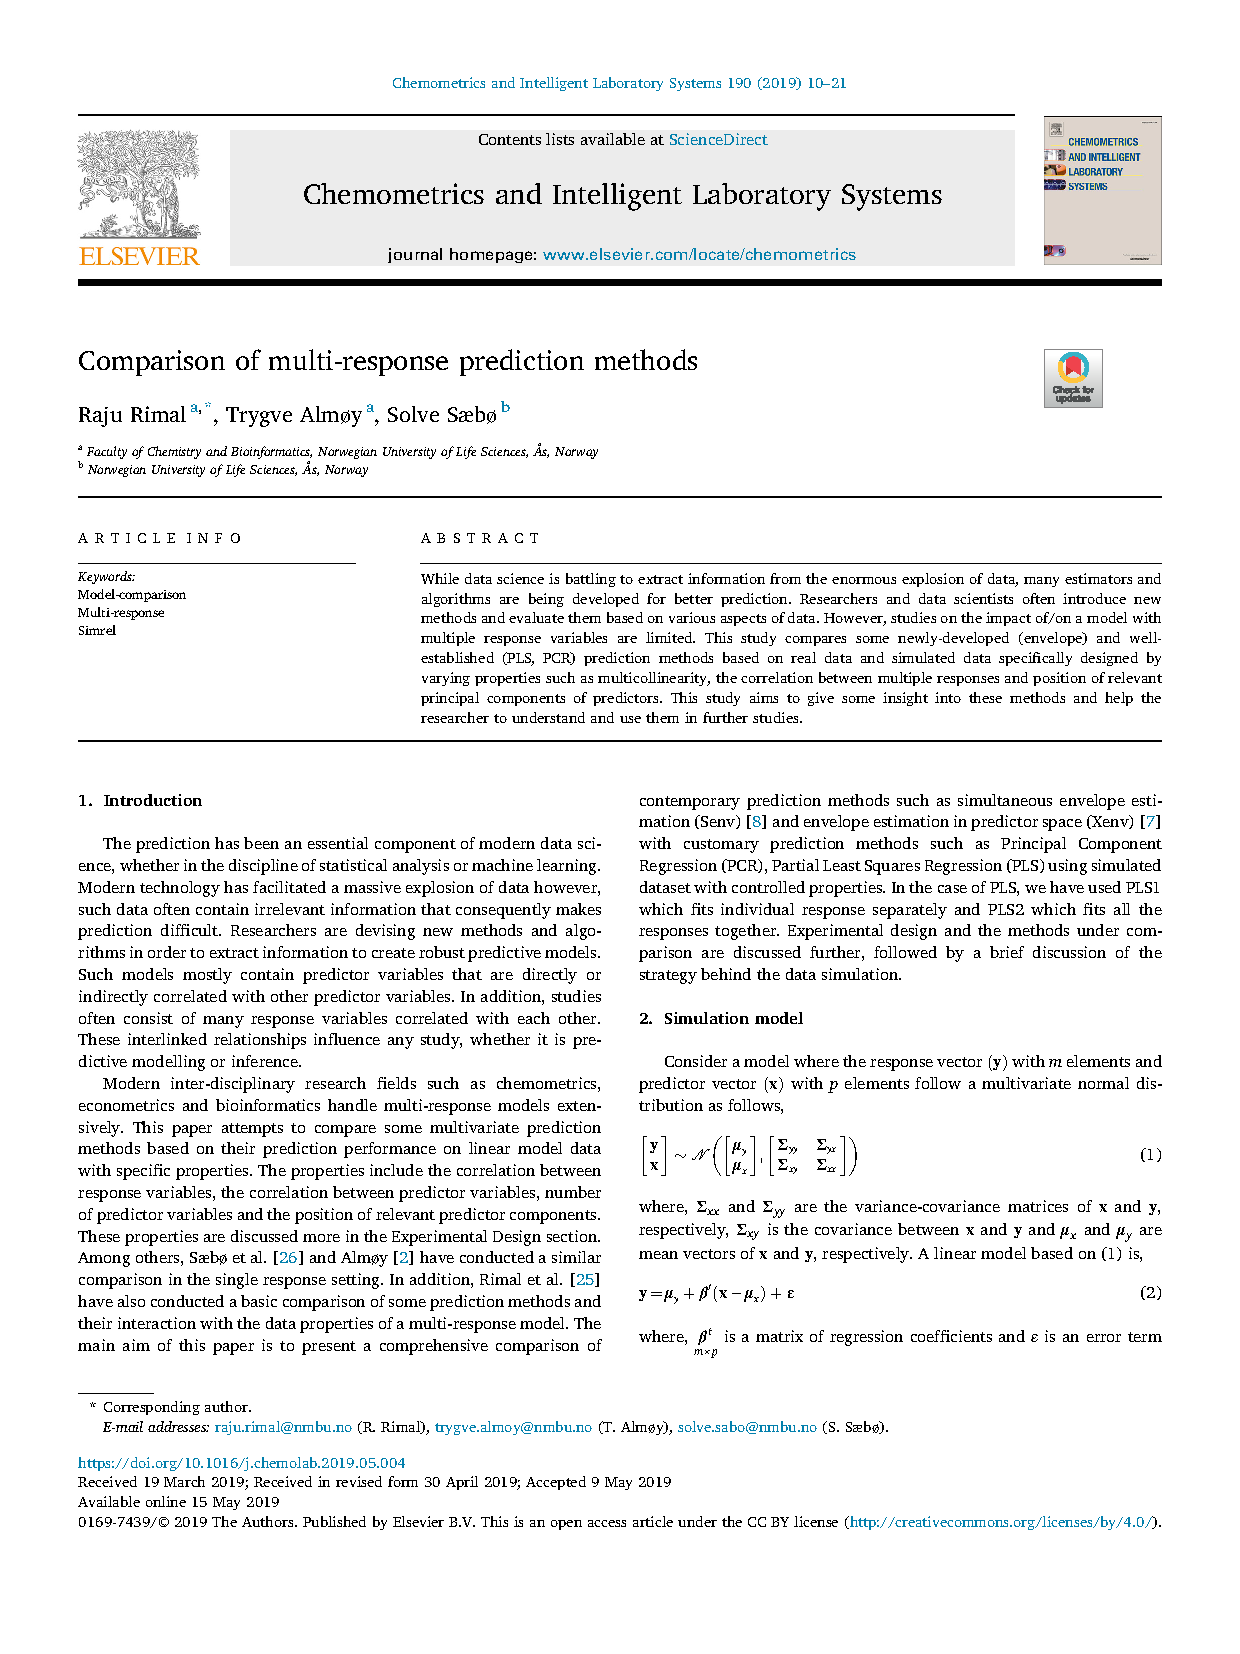
\includepdf[pages=-]{papers/003.pdf}

% *******************************************************
% ANYTHING EXTRA
% *******************************************************
$for(include-after)$
$include-after$
$endfor$

\end{document}

%%% Local Variables:
%%% mode: latex
%%% TeX-master: t
%%% End:
